\documentclass[a4paper]{article}
\usepackage{geometry}
\usepackage{graphicx}
\usepackage{natbib}
\usepackage{amsmath}
\usepackage{amssymb}
\usepackage{amsthm}
\usepackage{paralist}
\usepackage{epstopdf}
\usepackage{tabularx}
\usepackage{longtable}
\usepackage{multirow}
\usepackage{multicol}
\usepackage[hidelinks]{hyperref}
\usepackage{fancyvrb}
\usepackage{algorithm}
\usepackage{algorithmic}
\usepackage{float}
\usepackage{paralist}
\usepackage[svgname]{xcolor}
\usepackage{enumerate}
\usepackage{array}
\usepackage{times}
\usepackage{url}
\usepackage{fancyhdr}
\usepackage{comment}
\usepackage{environ}
\usepackage{times}
\usepackage{textcomp}
\usepackage{caption}
\usepackage{bbm}
\usepackage{enumitem}
\usepackage{subcaption}

\urlstyle{rm}

\setlength\parindent{0pt} % Removes all indentation from paragraphs
\theoremstyle{definition}
\newtheorem{definition}{Definition}[]
\newtheorem{conjecture}{Conjecture}[]
\newtheorem{example}{Example}[]
\newtheorem{theorem}{Theorem}[]
\newtheorem{lemma}{Lemma}
\newtheorem{proposition}{Proposition}
\newtheorem{corollary}{Corollary}

\floatname{algorithm}{Procedure}
\renewcommand{\algorithmicrequire}{\textbf{Input:}}
\renewcommand{\algorithmicensure}{\textbf{Output:}}
\newcommand{\abs}[1]{\lvert#1\rvert}
\newcommand{\norm}[1]{\lVert#1\rVert}
\newcommand{\RR}{\mathbb{R}}
\newcommand{\CC}{\mathbb{C}}
\newcommand{\Nat}{\mathbb{N}}
\newcommand{\br}[1]{\{#1\}}
\DeclareMathOperator*{\argmin}{arg\,min}
\DeclareMathOperator*{\argmax}{arg\,max}
\renewcommand{\qedsymbol}{$\blacksquare$}

\definecolor{dkgreen}{rgb}{0,0.6,0}
\definecolor{gray}{rgb}{0.5,0.5,0.5}
\definecolor{mauve}{rgb}{0.58,0,0.82}

\newcommand{\Var}{\mathrm{Var}}
\newcommand{\Cov}{\mathrm{Cov}}

\newcommand{\vc}[1]{\boldsymbol{#1}}
\newcommand{\xv}{\vc{x}}
\newcommand{\Sigmav}{\vc{\Sigma}}
\newcommand{\alphav}{\vc{\alpha}}
\newcommand{\muv}{\vc{\mu}}

\newcommand{\red}[1]{\textcolor{red}{#1}}
\newcommand{\blue}[1]{\textcolor{blue}{#1}}

\def\x{\mathbf x}
\def\y{\mathbf y}
\def\w{\mathbf w}
\def\v{\mathbf v}
\def\E{\mathbb E}
\def\V{\mathbb V}
\def\ind{\mathbbm 1}

% TO SHOW SOLUTIONS, include following (else comment out):
\newenvironment{soln}{
    \leavevmode\color{blue}\ignorespaces
}{}


\hypersetup{
%    colorlinks,
    linkcolor={red!50!black},
    citecolor={blue!50!black},
    urlcolor={blue!80!black}
}

\geometry{
  top=1in,            % <-- you want to adjust this
  inner=1in,
  outer=1in,
  bottom=1in,
  headheight=3em,       % <-- and this
  headsep=2em,          % <-- and this
  footskip=3em,
}


\pagestyle{fancyplain}
\lhead{\fancyplain{}{Homework 4}}
\rhead{\fancyplain{}{CS 760 Machine Learning}}
\cfoot{\thepage}

\title{\textsc{Homework 4}} % Title

%%% NOTE:  Replace 'NAME HERE' etc., and delete any "\red{}" wrappers (so it won't show up as red)

\author{
Saikumar Yadugiri\\
9083079468, saikumar@cs.wisc.edu\\
} 

\date{}

\begin{document}

\maketitle 


\textbf{Instructions:} Use this latex file as a template to develop your homework. Submit your homework on time as a single pdf file to Canvas. Late submissions may not be accepted. Please wrap your code and upload to a public GitHub repo, then attach the link below the instructions so that we can access it. You can choose any programming language (i.e. python, R, or MATLAB). Please check Piazza for updates about the homework.

\paragraph{GitHub Link} \href{https://github.com/saikumarysk/cs760_hw4}{\texttt{https://github.com/saikumarysk/cs760\_hw4}}

\section{Best Prediction Under 0-1 Loss (10 pts)}
Suppose the world generates a single observation $x \sim \mbox{multinomial}(\theta)$, where the parameter vector $\theta=(\theta_1, \ldots, \theta_k)$ with $\theta_i\ge 0$ and $\sum_{i=1}^k \theta_i=1$.  Note $x \in \{1, \ldots, k\}$.
You know $\theta$ and want to predict $x$. 
Call your prediction $\hat x$.  What is your expected 0-1 loss: 
$$\E[\ind_{\hat x \neq x}]$$
using the following two prediction strategies respectively?  Prove your answer.


Strategy 1: $\hat x \in \argmax_x \theta_x$, the outcome with the highest probability.

\begin{soln}
    As this strategy is deterministic, there is no randomness in the choice of $\hat{x}$. So, the expectation is taken on the world's prediction. Note that the values of $\hat{x}$ can be several as $\argmax$ gives a set of values. However, as we need a single prediction to match the world's observation, we take some fixed value in that set. Then,

    \begin{equation*}
        \E [\ind_{\hat{x} \neq x}] = \sum\limits_{x} \Pr [\hat{x} \neq x] = 1 -  \Pr [\hat{x} = x] = 1 - \theta_{\hat{x}}
    \end{equation*}
\end{soln}

Strategy 2: You mimic the world by generating a prediction $\hat x \sim \mbox{multinomial}(\theta)$.  (Hint: your randomness and the world's randomness are independent)

\begin{soln}
    Now, we have some randomness in the choice of $\hat{x}$. Similar to above, we have

    \begin{align*}
        \E [\ind_{\hat{x} \neq x}] &= \Pr [\hat{x} \neq x] \\
        &= \sum\limits_{i = 1}^{k} \Pr [x \neq \hat{x} \mid \hat{x} = i] \Pr [\hat{x} = i] \\
        &= \sum\limits_{i = 1}^{k} \Pr [x \neq i] \Pr [\hat{x} = i] \\
        &= \sum\limits_{i = 1}^{k} (1 - \theta_i) \theta_i \\
        &= 1 - \sum\limits_{i = 1}^{k} \theta_i^2
    \end{align*}
\end{soln}
\pagebreak

\section{Best Prediction Under Different Misclassification Losses (6 pts)}
Like in the previous question, 
the world generates a single observation $x \sim \mbox{multinomial}(\theta)$.
Let $c_{ij} \ge 0$ denote the loss you incur, if $x=i$ but you predict $\hat x=j$, for $i,j \in \{1, \ldots, k\}$.
$c_{ii}=0$ for all $i$.
This is a way to generalize different costs on false positives vs false negatives from binary classification to multi-class classification.
You want to minimize your expected loss:
$$\E[c_{x \hat x}]$$
Derive your optimal prediction $\hat x$.

\begin{soln}
    If we do not know the values of $c_{ij}$ a-priori, we can calculate them or stick to the strategies in the previous question. So, I am assuming that we know the matrix $\mathbf{C} = [c_{ij}]_{ij}$ a-priori but not the world's observation. As we do not know $x$, we can choose a randomized prediction a la strategy 2 in previous question, by choosing $\hat{x}$ from a multinomial distribution as well. Then,

    \begin{align*}
        \E [c_{x\hat{x}}] &= \sum\limits_{i=1}^{k} \sum\limits_{j=1}^{k} c_{ij} \Pr [x = i] \Pr [x = j] \\
        &= \sum\limits_{i \neq j} c_{ij} \theta_i \theta_j
    \end{align*}

    We need to minimize this loss. Hence, we need $\argmin\limits_{j} \E [c_{x \hat{x}} \mid \hat{x} = j] = \argmin\limits_{j} \sum\limits_{i \neq j} c_{ij} \theta_i$. So, our prediction $\hat{x} = \argmin\limits_{j} \sum\limits_{i \neq j} c_{ij} \theta_i$.
    
\end{soln}
\pagebreak


\section{Language Identification with Naive Bayes (8 pts each)}
Implement a character-based Naive Bayes classifier that classifies a document as English, Spanish, or Japanese - all written with the 26 lower case characters and space.

The dataset is languageID.tgz, unpack it.
This dataset consists of 60 documents in English, Spanish and Japanese. 
The correct class label is the first character of the filename: $y \in \{e, j, s\}$. (Note: here each file is a document in corresponding language, and it is regarded as one data.)

We will be using a character-based multinomial Naïve Bayes model.  You need to view each document as a bag of characters, including space.  We have made sure that there are only 27 different types of printable characters (a to z, and space) -- there may be additional control characters such as new-line, please ignore those.  Your vocabulary will be these 27 character types. (Note: not word types!)


\begin{enumerate}
\item
Use files 0.txt to 9.txt in each language as the training data.
Estimate the prior probabilities 
$\hat p(y=e)$,
$\hat p(y=j)$,
$\hat p(y=s)$
using additive smoothing with parameter $\frac{1}{2}$. 
Give the formula for additive smoothing with parameter $\frac{1}{2}$ in this case. 
Print and include in final report the prior probabilities.
(Hint: Store all probabilities here and below in $\log()$ internally to avoid underflow. This also means you need to do arithmetic in log-space.  But answer questions with probability, not log probability.)

\begin{soln}
    The formula for the prior probabilities are given by

    \begin{align*}
        \hat{p} \left[ y = e \right] &= \frac{\left( \sum\limits_{i=1}^{N} \ind \left[ y^{(i)} = e \right] \right) + 0.5}{N + 1.5} \\
        \hat{p} \left[ y = s \right] &= \frac{\left( \sum\limits_{i=1}^{N} \ind \left[ y^{(i)} = s \right] \right) + 0.5 }{N + 1.5} \\
        \hat{p} \left[ y = j \right] &= \frac{\left( \sum\limits_{i=1}^{N} \ind \left[ y^{(i)} = j \right] \right) + 0.5 }{N + 1.5}
    \end{align*}

    From my calculations, I got $\hat{p} \left[ y = e \right] = 0.33333$, $\hat{p} \left[ y = s \right] = 0.33333$, and $\hat{p} \left[ y = j \right] = 0.33333$.
\end{soln}

\pagebreak
\item
Using the same training data, estimate the class conditional probability (multinomial parameter) for English
$$\theta_{i,e} := \hat p(c_i \mid y=e)$$ 
where $c_i$ is the $i$-th character. That is, $c_1 = a, \ldots, c_{26} = z, c_{27} = space$.
Again use additive smoothing with parameter $\frac{1}{2}$.
Give the formula for additive smoothing with parameter $\frac{1}{2}$ in this case. 
Print $\theta_e$ and include in final report which is a vector with 27 elements.

\begin{soln}
    The formula is given by

    \begin{equation*}
        \theta_{i, e} = \hat{p} \left[ c_i \mid y = e \right] = \frac{\left( \sum\limits_{j=1}^{N} \sum\limits_{k = 1}^{M_j} \ind \left[ x_k^{(j)} = c_i, y^{(j)} = e \right] \right) + 0.5}{\left( \sum\limits_{c \in C} \sum\limits_{j=1}^{N} \sum\limits_{k = 1}^{M_j} \ind \left[ x_k^{(j)} = c, y^{(j)} = e \right] \right) + 1.5}
    \end{equation*}

     where $M_j$ is the number of characters in the $j$-th file for english language, $x^{(j)}_k$ is the $k$-th character in the $j$-th file for english, and $C$ is the set of 27 characters, i.e, $a-z$ and space. The conditional probabilities are shown in table \ref{tab:1}.
    
    \begin{table}[H]
        \centering
        \begin{tabular}{|c|c|c|c|c|c|}
            \hline
            \multicolumn{6}{|c|}{$\theta_e$}\\
            \hline
            a & 0.06017 & j & 0.00142 & s & 0.06618\\
            \hline
            b & 0.01113 & k & 0.00373 & t & 0.08013\\
            \hline
            c & 0.02151 & l & 0.02898 & u & 0.02666\\
            \hline
            d & 0.02197 & m & 0.02052 & v & 0.00928\\
            \hline
            e & 0.10537 & n & 0.05792 & w & 0.0155\\
            \hline
            f & 0.01893 & o & 0.06446 & x & 0.00116\\
            \hline
            g & 0.01748 & p & 0.01675 & y & 0.01384\\
            \hline
            h & 0.04722 & q & 0.00056 & z & 0.00063\\
            \hline
            i & 0.05541 & r & 0.05382 & space & 0.17925\\
            \hline
        \end{tabular}
        \caption{Likelihood for English files}
        \label{tab:1}
    \end{table}
\end{soln}
\pagebreak

\item
Print $\theta_j, \theta_s$ and include in final report the class conditional probabilities for Japanese and Spanish.

\begin{soln}
    The required conditional probabilities are shown in tables \ref{tab:2} and \ref{tab:3}.
    \begin{table}[H]
        \centering
        \begin{tabular}{|c|c|c|c|c|c|}
            \hline
            \multicolumn{6}{|c|}{$\theta_s$}\\
            \hline
            a & 0.13177 & j & 0.00234 & s & 0.04217 \\
            \hline
            b & 0.01087 & k & 0.05741 & t & 0.05699 \\
            \hline
            c & 0.00549 & l & 0.00143 & u & 0.07062 \\
            \hline
            d & 0.01723 & m & 0.0398 & v & 0.00024 \\
            \hline
            e & 0.0602 & n & 0.05671 & w & 0.01974 \\
            \hline
            f & 0.00388 & o & 0.09116 & x & 3e-05 \\
            \hline
            g & 0.01401 & p & 0.00087 & y & 0.01415 \\
            \hline
            h & 0.03176 & q & 0.0001 & z & 0.00772 \\
            \hline
            i & 0.09703 & r & 0.0428 & space & 0.12345 \\
            \hline
        \end{tabular}
        \caption{Likelihood for Japanese Files}
        \label{tab:2}%
        \begin{tabular}{|c|c|c|c|c|c|}
            \hline
            \multicolumn{6}{|c|}{$\theta_j$}\\
            \hline
            a & 0.10456 & j & 0.00663 & s & 0.06577 \\
            \hline
            b & 0.00823 & k & 0.00028 & t & 0.03561 \\
            \hline
            c & 0.03753 & l & 0.05294 & u & 0.0337 \\
            \hline
            d & 0.03975 & m & 0.02581 & v & 0.00589 \\
            \hline
            e & 0.11381 & n & 0.05418 & w & 9e-05 \\
            \hline
            f & 0.0086 & o & 0.07249 & x & 0.0025 \\
            \hline
            g & 0.00718 & p & 0.02427 & y & 0.00786 \\
            \hline
            h & 0.00453 & q & 0.00768 & z & 0.00268 \\
            \hline
            i & 0.04986 & r & 0.0593 & space & 0.16826 \\
            \hline
        \end{tabular}
        \caption{Likelihood for Spanish files}
        \label{tab:3}
    \end{table}
\end{soln}
\pagebreak

\item
Treat e10.txt as a test document $x$.
Represent $x$ as a bag-of-words count vector (Hint: the vocabulary has size 27).
Print the bag-of-words vector $x$ and include in final report.

\begin{soln}
    The vector can be found in table \ref{tab:4}.
    \begin{soln}
    \begin{table}[H]
        \centering
        \begin{tabular}{|c|c|c|c|c|c|}
            \hline
            \multicolumn{6}{|c|}{$x_{e10}$}\\
            \hline
            a & 164 & j & 3 & s & 186 \\
            \hline
            b & 32 & k & 6 & t & 225 \\
            \hline
            c & 53 & l & 85 & u & 65 \\
            \hline
            d & 57 & m & 64 & v & 31 \\
            \hline
            e & 311 & n & 139 & w & 47 \\
            \hline
            f & 55 & o & 182 & x & 4 \\
            \hline
            g & 51 & p & 53 & y & 38 \\
            \hline
            h & 140 & q & 3 & z & 2 \\
            \hline
            i & 140 & r & 141 & space & 498 \\
            \hline
        \end{tabular}
        \caption{Bag of Words Vector for \textsf{e10.txt}}
        \label{tab:4}
    \end{table}
\end{soln}
\end{soln}
\pagebreak

\item
Compute $\hat p(x \mid y)$ for $y=e, j, s$ under the multinomial model assumption, respectively.
Use the formula
$$\hat p(x \mid y) = \prod_{i=1}^d \theta_{i, y}^{x_i}$$
where $x=(x_1, \ldots, x_d)$.
Show the three values: $\hat p(x \mid y=e), \hat p(x \mid y=j), \hat p(x \mid y=s)$.
Hint: you may notice that we omitted the multinomial coefficient.  This is ok for classification because it is a constant w.r.t. $y$.

\begin{soln}
    The conditional probabilities are really low. So, I am printing $\log_{10}(\cdot)$ of these probabilities.

    \begin{align*}
        \log_{10}(\hat{p}(x \mid y = e)) &= -3405.70056\\
        \log_{10}(\hat{p}(x \mid y = j)) &= -3810.12905\\
        \log_{10}(\hat{p}(x \mid y = s)) &= -3677.90439
    \end{align*}
\end{soln}
\pagebreak

\item
Use Bayes rule and your estimated prior and likelihood, compute the posterior $\hat p(y \mid x)$.
Show the three values: $\hat p(y=e \mid x), \hat p(y=j \mid x), \hat p(y=s \mid x)$.
Show the predicted class label of $x$.

\begin{soln}
    As we do not know $\hat{p}(x)$, we can use $\hat{p}(x | y) \times \hat{p}(y)$ as a proxy for the posterior probability $\hat{p}(y | x)$. This is because posterior probability is the product of likelihood and prior probabilities. As likelihood probabilities are really low, I am use $\log_{10}(\cdot)$ to show posterior probabilities as well.

    \begin{align*}
        \hat{p}(y = e | x) &\propto \log_{10}(\hat{p}(x | y = e)) + \log_{10}(\hat{p}(y = e)) = -3406.17768 \\
        \hat{p}(y = j | x) &\propto \log_{10}(\hat{p}(x | y = j)) + \log_{10}(\hat{p}(y = j)) = -3810.60617 \\
        \hat{p}(y = s | x) &\propto \log_{10}(\hat{p}(x | y = s)) + \log_{10}(\hat{p}(y = s)) = -3678.38151
    \end{align*}

    The highest value in all the posterior probabilities will be our prediction from classifier. Hence, the prediction is \textsf{english}.
\end{soln}
\pagebreak

\item
Evaluate the performance of your classifier on the test set (files 10.txt to 19.txt in three languages).
Present the performance using a confusion matrix. A confusion matrix summarizes the types of errors your classifier makes, as shown in the table below.   The columns are the true language a document is in, and the rows are the classified outcome of that document.  The cells are the number of test documents in that situation.  For example, the cell with row = English and column = Spanish contains the number of test documents that are really Spanish, but misclassified as English by your classifier.

\begin{soln}
    The confusion matrix can be found in table \ref{tab:5}.
    \begin{table}[H]
        \centering
        \begin{tabular}{|c|c|c|c|}
            \hline
             & English & Japanese & Spanish \\
            \hline
            English & 10 & 0 & 0 \\
            \hline
            Japanese & 0 & 10 & 0 \\
            \hline
            Spanish & 0 & 0 & 10 \\
            \hline
        \end{tabular}
        \caption{Confusion Matrix for Testing Data}
        \label{tab:5}
    \end{table}
\end{soln}
\pagebreak

\item If you take a test document and arbitrarily shuffle the order of its characters so that the words (and spaces) are scrambled beyond human recognition.  How does this shuffling affect your Naive Bayes classifier's prediction on this document?  Explain the key mathematical step in the Naive Bayes model that justifies your answer.

\begin{soln}
    The arbitrary shuffling does not affect classifier's prediction. This is because the formulae for calculating the prior and likelihood probabilities are just counting the number of files or number of characters in each file respectively. In other words, we are predicting using character frequency in each language. So, shuffling of characters will not change the character frequency. Even if you insert additional characters which are not in the set $\{a-z, \text{space}\}$, we will not see any changes in the classifier's prediction.
\end{soln}

\end{enumerate}
\pagebreak

\section{Simple Feed-Forward Network (20pts)}
In this exercise, you will derive, implement back-propagation for a simple neural network and compare your output with some standard library’s output. Consider the following 3-layer neural network.

\[
\hat{y} = f(x) = g(W_2\sigma(W_1x))
\]

Suppose $x \in \mathbb{R}^d$, $W_1 \in \mathbb{R}^{d_1 \times d}$, and $W_2 \in \mathbb{R}^{k \times d_1}$ i.e. $f: \mathbb{R}^d \rightarrow \mathbb{R}^k$, Let $\sigma(z) = [\sigma(z_1), ..., \sigma(z_n)]$ for any $z \in \mathbb{R}^n$ where $\sigma(z) = \frac{1}{1 + e^{-z}}$ is the sigmoid (logistic) activation function and $g(z_i) = \frac{exp(z_i)}{\sum_{i=1}^k exp(z_i)}$ is the softmax function. Suppose the true pair is $(x, y)$ where $y \in \{0, 1\}^k$ with exactly one of the entries equal to 1, and you are working with the cross-entropy loss function given below,

\[
L(x, y) = -\sum_{l=1}^k y \text{log}(\hat{y})
\]

\begin{enumerate}
    \item Derive backpropagation updates for the above neural network. (5 pts) \\
    \begin{soln}
    Consider the derivative w.r.to $W_2$ first as it will be easier to derive. Let's denote $W_2 = \left[ w_{ij}^{(2)} \right]_{ij}$. Now, by chain rule,

    \begin{equation*}
        \frac{\partial L(x, y)}{\partial w_{ij}^{(2)}} = - \sum\limits_{l = 1}^{k} \frac{y_l}{\hat{y}_l} \left( \sum\limits_{m = 1}^{k} \frac{\partial \hat{y}_l}{\partial z_m} \frac{\partial z_m}{\partial w_{ij}^{(2)}} \right)
    \end{equation*}

    where $z_m$ is the linear input to the output neuron, i.e, $z_m = w_{m1}^{(2)} a_{1} + \ldots + w_{m d_1}^{(2)} a_{d_1}$ (where the bias term is implicit in the linear term) and $a_{i}$ is the activation of the hidden layer's neurons. Now, $\frac{\partial z_m}{\partial w_{ij}^{(2)}} = a_{j}$ if $m = i$ and $0$ otherwise. So,

    \begin{align*}
        \frac{\partial L(x, y)}{\partial w_{ij}^{(2)}} &= - \sum\limits_{l = 1}^{k} \frac{y_l}{\hat{y}_l} a_{j} \frac{\partial \hat{y}_l}{\partial z_i}, \\
        \frac{\partial \hat{y}_i}{\partial z_i} &= \frac{\left( \sum\limits_{l = 1}^{k} e^{z_l} \right) e^{z_i} - e^{2z_i} }{\left( \sum\limits_{l = 1}^{k} e^{z_l} \right)^2} \\
        &= \hat{y}_i (1 - \hat{y}_i) \\
        \frac{\partial \hat{y}_l}{\partial z_i} &= \frac{\left( \sum\limits_{m = 1}^{k} e^{z_m} \right) \cdot 0 - e^{z_i} e^{z_l} }{\left( \sum\limits_{m = 1}^{k} e^{z_m} \right)^2} \quad (l \neq i) \\
        &= -\hat{y}_l \hat{y}_i \\
        \implies \frac{\partial L(x, y)}{\partial w_{ij}^{(2)}} &= - y_i (1- \hat{y}_i) a_j + \sum\limits_{l \neq i} y_l \hat{y}_i a_j \\
        &= -y_ia_j + \left(\sum_{l = 1}^{k} y_l \right) \hat{y}_i a_j \\
        \frac{\partial L(x, y)}{\partial w_{ij}^{(2)}} &= (\hat{y}_i - y_i) a_j
    \end{align*}

    The last step comes because this is a classification task, $y$ can be thought of as a one-hot vector. Finally, we can write,

    \begin{equation*}
        \frac{\partial L(x, y)}{\partial W_2} = (\hat{y} - y) a^{T} \quad (\text{outer product})
    \end{equation*}
    
    Now let's derive backpropogation updates for $W_1 = \left[ w_{ij}^{(1)} \right]_{ij}$. By chain rule,

    \begin{equation*}
        \frac{\partial L(x, y)}{\partial w_{ij}^{(1)}} = - \sum\limits_{l = 1}^{k} \frac{y_l}{\hat{y}_l} \left( \sum\limits_{m = 1}^{k} \frac{\partial \hat{y}_l}{\partial z_m} \frac{\partial z_m}{\partial w_{ij}^{(1)}} \right)
    \end{equation*}

    where $z_m$ is same as described above. In $z_m$, the only place which $w_{ij}^{(1)}$ appears is in the neuron for $a_i$. So, $\frac{\partial z_m}{\partial w_{ij}^{(1)}} = w_{mi}^{(2)} \frac{\partial a_i}{\partial w_{ij}^{(1)}}$.

    \begin{align*}
        \frac{\partial a_i}{\partial w_{ij}^{(1)}} = a_i(1 - a_i) \frac{\partial \tilde{z_i}}{\partial w_{ij}^{(i)}}
    \end{align*}

    where $\tilde{z_i} = w_{i1}^{(1)}x_1 + \ldots + w_{i d}^{(1)} x_d$. This is because $a_i$ is the activation of first hidden layer using the sigmoid function and $\sigma^\prime(z) = \sigma(z)(1 - \sigma(z))$. Hence, $\frac{\partial \tilde{z_i}}{\partial w_{ij}^{(i)}} = x_j$.

    \begin{align*}
        \frac{\partial L(x, y)}{\partial w_{ij}^{(1)}} &= - \sum\limits_{l = 1}^{k} \frac{y_l}{\hat{y}_l} \left( \sum\limits_{m = 1}^{k} \frac{\partial \hat{y}_l}{\partial z_m} w_{mi}^{(2)} a_i (1 - a_i) x_j \right) \\
        &= - a_i (1 - a_i) x_j \sum\limits_{l = 1}^{k} \frac{y_l}{\hat{y}_l} \left( \sum\limits_{m = 1}^{k} \frac{\partial \hat{y}_l}{\partial z_m} w_{mi}^{(2)} \right) \\
        &= - a_i (1 - a_i) x_j \sum\limits_{l = 1}^{k} \frac{y_l}{\hat{y}_l} \left( \hat{y}_l (1 - \hat{y}_l) w_{li}^{(2)} - \sum\limits_{m \neq l} \hat{y}_l \hat{y}_m w_{mi}^{(2)} \right) \\
        &= - a_i (1 - a_i) x_j \sum\limits_{l = 1}^{k} y_l \left( w_{li}^{(2)} - \sum\limits_{m = 1}^{k} \hat{y}_m w_{mi}^{(2)} \right) \\
        &= - a_i (1 - a_i) x_j \sum\limits_{l = 1}^{k} y_l w_{li}^{(2)} - \left( \sum\limits_{l = 1}^{k} y_l \right) \left(\sum\limits_{m = 1}^{k} \hat{y}_m w_{mi}^{(2)} \right) \\
        &= - a_i (1 - a_i) x_j \left( \sum\limits_{l = 1}^{k} y_l w_{li}^{(2)} - \sum\limits_{m = 1}^{k} \hat{y}_m w_{mi}^{(2)} \right) \\
        \implies \frac{\partial L(x, y)}{\partial w_{ij}^{(1)}} &= \left( \sum\limits_{l = 1}^{k} (\hat{y}_l - y_l) w_{li}^{(2)} \right) a_i (1 - a_i) x_j
    \end{align*}

    This can be written using $\ast$ as element-wise multiplication,

    \begin{equation*}
        \frac{\partial L(x, y)}{\partial W_1} = \left( \left( W_2^T (\hat{y} - y) \right) \ast a \ast (1 - a) \right) x^T
    \end{equation*}
    
    \end{soln}

    \pagebreak
    
    \item Implement it in NumPy or PyTorch using basic linear algebra operations. (e.g. You are not allowed to use auto-grad, built-in optimizer, model, etc. in this step. You can use library functions for data loading, processing, etc.). Evaluate your implementation on MNIST dataset, report test errors and learning curve. (10 pts)

    \begin{soln}
        My implementation was 94.48\% accurate. This means the test error is 5.52\%. I used random weights from a normal distribution $\mathcal{N}(0, 0.01)$ as they provided the better accuracy. I trained for 10 epochs and the learning curve can be found in figure \ref{fig:1}.

        \begin{figure}[H]
            \centering
            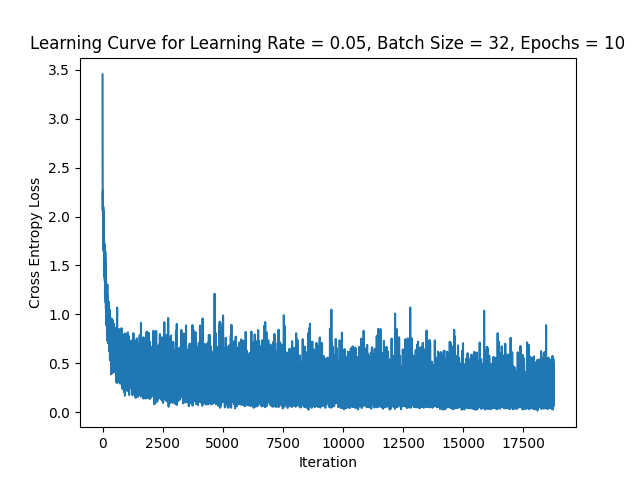
\includegraphics{MNIST_Learning_Curve_Self_Random.png}
            \caption{Learning Curve for MNIST Dataset on From Scratch Implementation of Neural Network}
            \label{fig:1}
        \end{figure}
    \end{soln}
    \pagebreak
    
    \item Implement the same network in PyTorch (or any other framework). You can use all the features of the framework e.g. auto-grad etc. Evaluate it on MNIST dataset, report test errors, and learning curve. (2 pts)
    
    \begin{soln}
        The accuracy of the implementation was 91.71\%. This means the test error is 8.29\%. I used random weights from a normal distribution $\mathcal{N}(0, 0.01)$ just like the previous question. I trained for 10 epochs and the learning curve can be found in figure \ref{fig:2}.

        \begin{figure}[H]
            \centering
            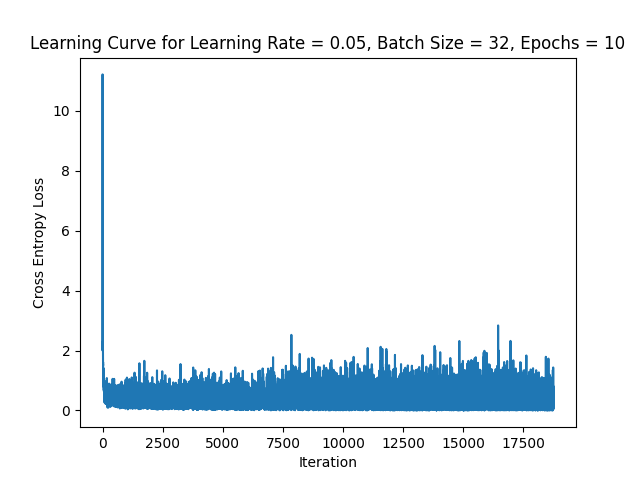
\includegraphics{MNIST_Learning_Curve_Torch_Random.png}
            \caption{Learning Curve for MNIST Dataset on From Scratch Implementation of Neural Network}
            \label{fig:2}
        \end{figure}
    \end{soln}
    
    \pagebreak
    
    \item Try different weight initialization a) all weights initialized to 0, and b) initialize the weights randomly between -1 and 1. Report test error and learning curves for both. (You can use either of the implementations) (3 pts)

    \begin{soln}
        The test error results can be found in table \ref{tab:6}. The learning curves can be found in figure \ref{fig:3}.
        \begin{table}[H]
            \centering
            \begin{tabular}{|c|c|c|}
                \hline
                 & Zero Weights & Random Weights \\
                \hline
                Scratch & 21.22 \% & 5.52 \% \\
                \hline
                PyTorch & 7.74 & 8.29 \% \\
                \hline
            \end{tabular}
            \caption{Test Errors in Percentage (\%) for My Implementations}
            \label{tab:6}
        \end{table}
        \begin{figure}[H]
            \centering
            \begin{subfigure}{0.5\textwidth}
              \centering
              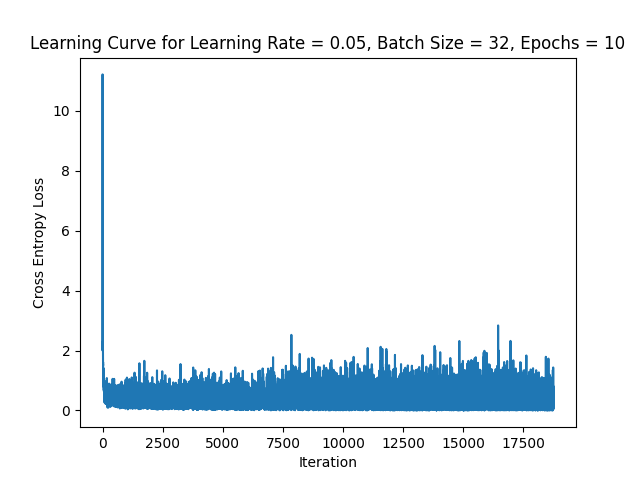
\includegraphics[width=1.1\linewidth]{MNIST_Learning_Curve_Torch_Random.png}
              \caption{Full PyTorch - Random Weights}
              \label{fig:3sub1}
            \end{subfigure}%
            \begin{subfigure}{0.5\textwidth}
              \centering
              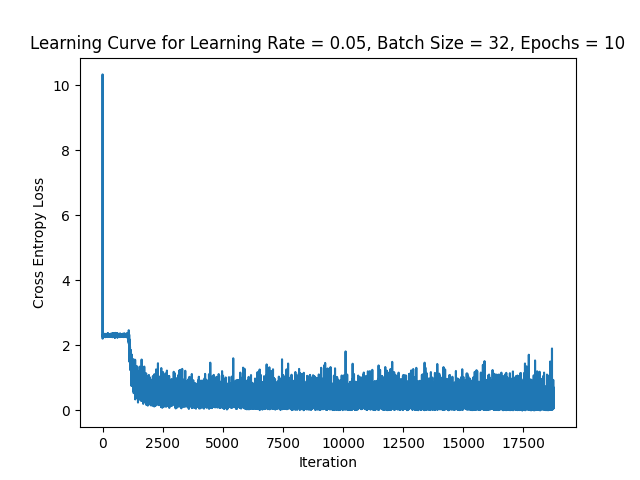
\includegraphics[width=1.1\linewidth]{MNIST_Learning_Curve_Torch_Zero.png}
              \caption{Full PyTorch - Zero Weights}
              \label{fig:3sub2}
            \end{subfigure}
            \begin{subfigure}{0.5\textwidth}
              \centering
              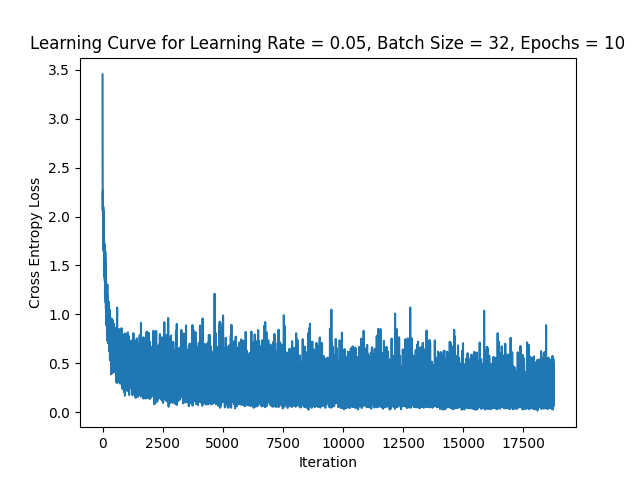
\includegraphics[width=1.1\linewidth]{MNIST_Learning_Curve_Self_Random.png}
              \caption{Scratch - Random Weights}
              \label{fig:3sub3}
            \end{subfigure}%
            \begin{subfigure}{0.5\textwidth}
              \centering
              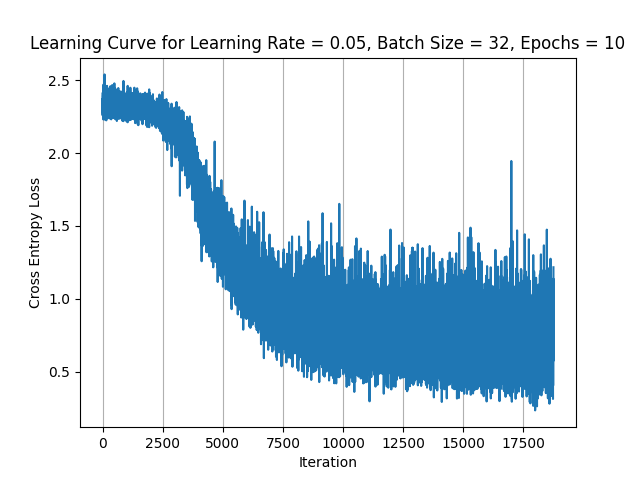
\includegraphics[width=1.1\linewidth]{MNIST_Learning_Curve_Self_Zero.png}
              \caption{Scratch - Zero Weights}
              \label{fig:3sub4}
              \end{subfigure}
            \caption{Zero Weights and Random Weights Learning Curves for Both My Implementations}
            \label{fig:3}
        \end{figure}
    \end{soln}
\end{enumerate}

You should play with different hyperparameters like learning rate, batch size, etc. for your own learning. You only need to report results for any particular setting of hyperparameters. You should mention the values of those along with the results. Use $d_1 = 300$ or $d_1 = 200$. For optimization use SGD (Stochastic gradient descent) without momentum, with some batch size say 32, 64, etc. MNIST can be obtained from here (https://pytorch.org/vision/ stable/datasets.html)

\bibliographystyle{apalike}
\end{document}